\documentclass[tikz]{standalone}

\usepackage{fontspec}

\usetikzlibrary{arrows}
\usetikzlibrary{calc}
\usetikzlibrary{decorations.pathreplacing}
\usetikzlibrary{positioning}
\usetikzlibrary{matrix}

\usepackage{fontspec}

\begin{document}

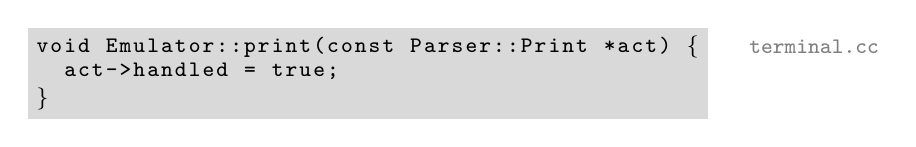
\begin{tikzpicture}
  [node distance=5mm, >=stealth',
  every node/.style={font=\footnotesize},
  every matrix/.style={fill=black!15, inner sep=1mm, row sep=0.5mm,
                        matrix of nodes, nodes in empty cells,
                        minimum height=0.5em, minimum width=.5em,
                        nodes={anchor=base, inner sep=0, font=\ttfamily\footnotesize}}]

  \matrix (snippet) {
v & o & i & d &   & E & m & u & l & a & t & o & r & : & : & p & r & i & n & t & ( & c & o & n & s & t &   & P & a & r & s & e & r & : & : & P & r & i & n & t &   & * & a & c & t & ) &   & \{ \\
  &   & a & c & t & - & > & h & a & n & d & l & e & d &   & = &   & t & r & u & e & ; &   &   &   &   &   &   &   &   &   &   &   &   &   &   &   &   &   &   &   &   &   &   &   &   &   &   \\
\} &   &   &   &   &   &   &   &   &   &   &   &   &   &   &   &   &   &   &   &   &   &   &   &   &   &   &   &   &   &   &   &   &   &   &   &   &   &   &   &   &   &   &   &   &   &   &   \\
  };

 \node [above, anchor=west, black!50, xshift=0.5cm]
        at (snippet-1-48.east)
        {\texttt{terminal.cc}};
\end{tikzpicture}

\end{document}
